\begin{frame}{Overview}

    % % \def\x{2mm}

% We extend \texttt{jim} \cite{wong2023fast}, based on \texttt{jax} \cite{jax2018github}, with building blocks:
% \vspace{2mm}
% \begin{enumerate}
%   % \item 
  
%   % \vspace{\x}

%   \item Normalizing flow-enhanced, gradient-based MCMC (\texttt{flowMC}, \cite{gabrie2021efficient, wong2022flowmc})
  
%   \vspace{\x}

%   \item Automatically-differentiable (AD) GW (\texttt{ripple} \cite{edwards2023ripple})
  
%   \vspace{\x}

%   \item \gray{Relative binning likelihood \cite{zackay2018relative}}
% \end{enumerate}

% \vspace{-3mm}

% \incfig[\textwidth]{jim_flowMC_ripple}
    \def\x{2mm}
  
  We extend \texttt{jim} \cite{wong2023fast}, based on \texttt{jax} \cite{jax2018github}, with building blocks:
  \vspace{2mm}
  \begin{enumerate}
    % \item 
    
    % \vspace{\x}
  
    \item Normalizing flow-enhanced, gradient-based MCMC (\texttt{flowMC}~\cite{gabrie2021efficient, wong2022flowmc})
    
    \vspace{\x}
  
    \item Automatically-differentiable (AD) GW (\texttt{ripple}~\cite{edwards2023ripple})
    
    \vspace{\x}
  
    \item \gray{Relative binning likelihood~\cite{zackay2018relative}}
  \end{enumerate}
  
  \vspace{-3mm}
  
  \incfig[\textwidth]{jim_flowMC_ripple}
    
  \end{frame}
  
  % % \section{Why \texttt{jax}?}
  
  % \begin{frame}{Why \texttt{jax}?}
  
  %   \def\x{4mm}
  
  %   \begin{tcolorbox}[colback=blue!10, boxrule=0pt]
  %     What are the benefits of \texttt{jax} for MCMC?
  %   \end{tcolorbox}
  
  % \vspace{3mm}
  
  % \begin{columns}
  %   \column{0.75\textwidth}
  %   \begin{enumerate}
  %     \item Automatic differentiation (AD)
      
  %     \vspace{\x}
  
  %     \item Just-in-time (JIT) compilation
      
  %     \vspace{\x}
      
  %     \item GPU acceleration
      
  %     \vspace{\x}
      
  %     \item Parallelization
      
  %     % \vspace{\x}
      
  %     % \item Vectorization
      
  %     % \vspace{\x}
      
  %     % \item Interoperability with \texttt{numpy}
  %   \end{enumerate}
  %   \column{0.20\textwidth}
  %   \begin{figure}
  %     % \centering
  %     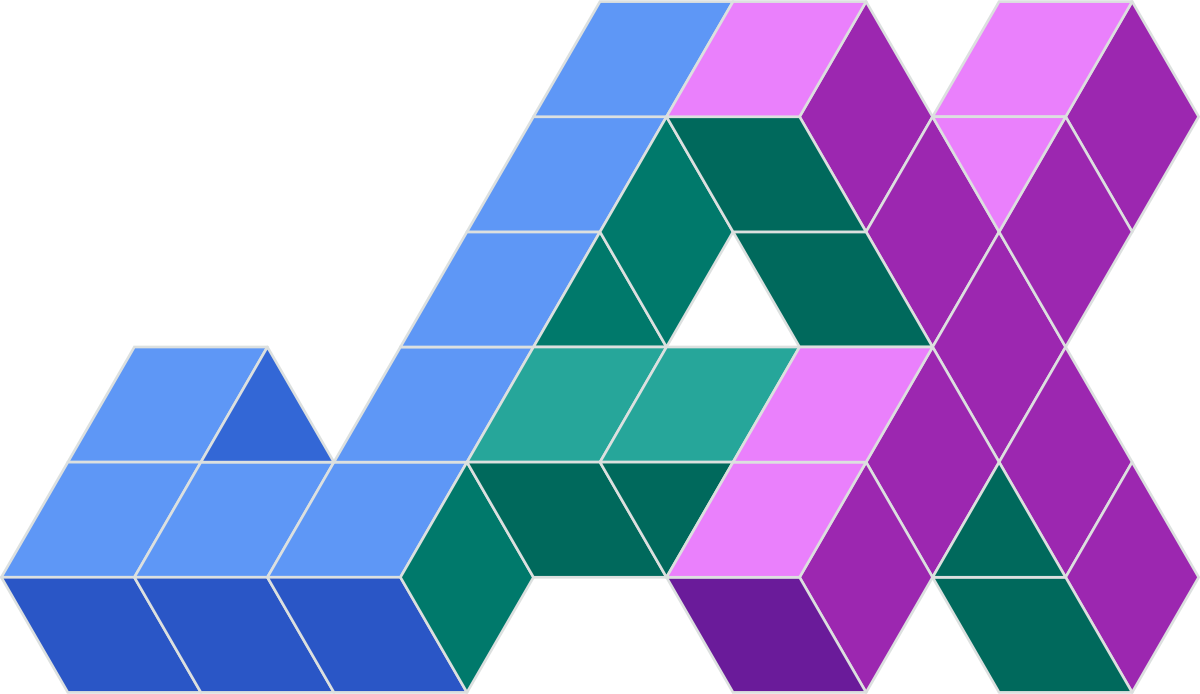
\includegraphics[width=\textwidth]{Figures/jax.png}
  %   \end{figure}
  % \end{columns}
    
  % \end{frame}
  
  % \section{\texttt{flowMC}}
  
  \begin{frame}{\texttt{flowMC} -- local sampling}
  
  \begin{enumerate}
    \item \textbf{Local sampling}: MALA (Metropolis-adjusted Langevin algorithm)
    
    \vspace{3mm}
    
    \begin{itemize}
      \item Proposal \red{$y$}: Langevin diffusion
      \begin{equation*}
        \red{y} = x + \frac{\epsilon^2}{2} \nabla \log p(x) + \epsilon \xi
      \end{equation*}
  
      \item Metropolis-Hastings acceptance step
      
      \vspace{3mm}

      \item Motivates the need for automatic differentiation
    \end{itemize}
    
  \end{enumerate}
  
  \incfig[\textwidth]{MALA}
  
  \end{frame}
  
  
  
  \begin{frame}{\texttt{flowMC} -- normalizing flows}
  
  \def\x{3mm}
  \def\y{5mm}
  
  Normalizing flows (NF):
  
  \vspace{\x}
  
  \begin{itemize}
    \item \blue{Latent space}: easy to sample (e.g. Gaussian)
    
    \vspace{\x}
  
    \item \red{Data space}: distribution learned from samples
    
    \vspace{\x}
    
    \item Enable approximate sampling from complicated distributions
  \end{itemize}
  
  \vspace{\y}
    
  \incfig[\textwidth]{NF}
  
  \end{frame}
  
  
  \begin{frame}{\texttt{flowMC} -- global sampling}
  
    \def\x{3mm}
    \def\y{2mm}
  
    \begin{enumerate}
      \setcounter{enumi}{1}
      \item \textbf{Global sampling}
    \end{enumerate}
  
    \vspace{\x}
  
    \begin{itemize}
      \item Global proposal by sampling from NF
      
      \vspace{\y}
      
      \item Metropolis-Hastings acceptance step
    \end{itemize}
  
    \vspace{8mm}
    
    \incfig[\textwidth]{global_sampling}
  
  \end{frame}
  
  
  
  \begin{frame}{\texttt{flowMC} -- complete algorithm}
  
    \only<1>{\textbf{Training loop} \& Production loop}
    \only<2>{Training loop \& \textbf{Production loop}}
  
    \vspace{-5mm}  
    
    \only<1>{
      \incfig[\textwidth]{flowMC_loop}
    }
  
    \only<2>{
      \vspace{1cm}
      \incfig[\textwidth]{flowMC_loop_production}
    }
  
  \end{frame}
  
  
  % \section{Results}
  
  \begin{frame}{Results}
    \def\x{2mm}
    \def\y{-3mm}
  
  
    % Tidal waveform models in \texttt{ripple}:
    \begin{itemize}
      \item TaylorF2 in \texttt{ripple}
      
      \vspace{\x}
  
      \item IMRPhenomD\_NRTidalv2 in \texttt{ripple} (ongoing)
      
      \vspace{\x}
      
      \item Reproduced PE for GW170817 \& GW190425 with TaylorF2
      
      \vspace{\x}
  
      \item $\sim 30$ mins training, $\sim 1$ min sampling
    \end{itemize}
  
    \vspace{\y}
  
    % \incfig[\textwidth]{jim_flowMC_ripple}
    \vspace{8mm}
    \begin{figure}[H]
      \centering
      % 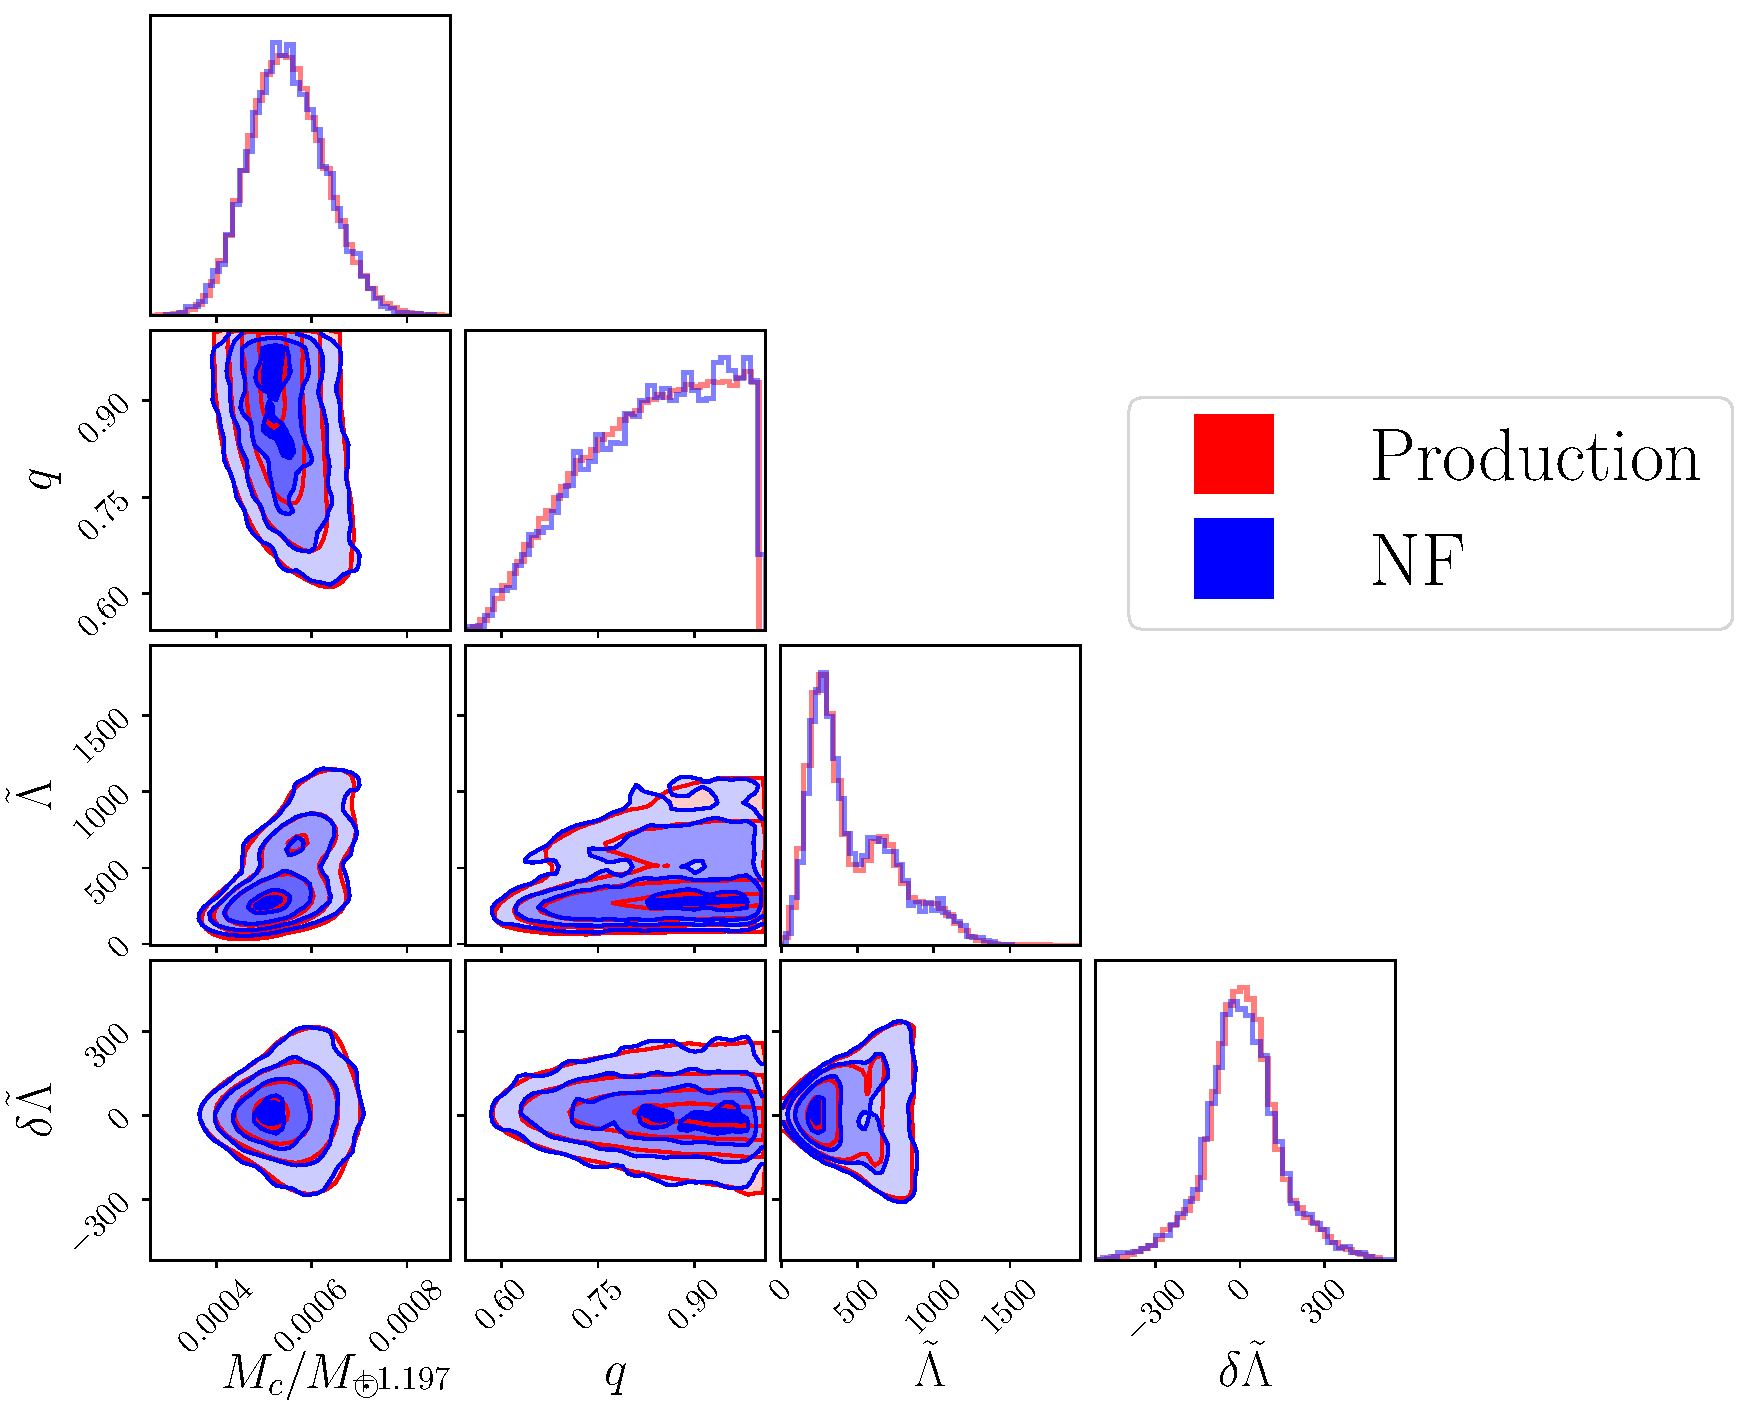
\includegraphics[scale=0.2]{Figures/presentation_GW170817_production_vs_NF_masses.pdf}
      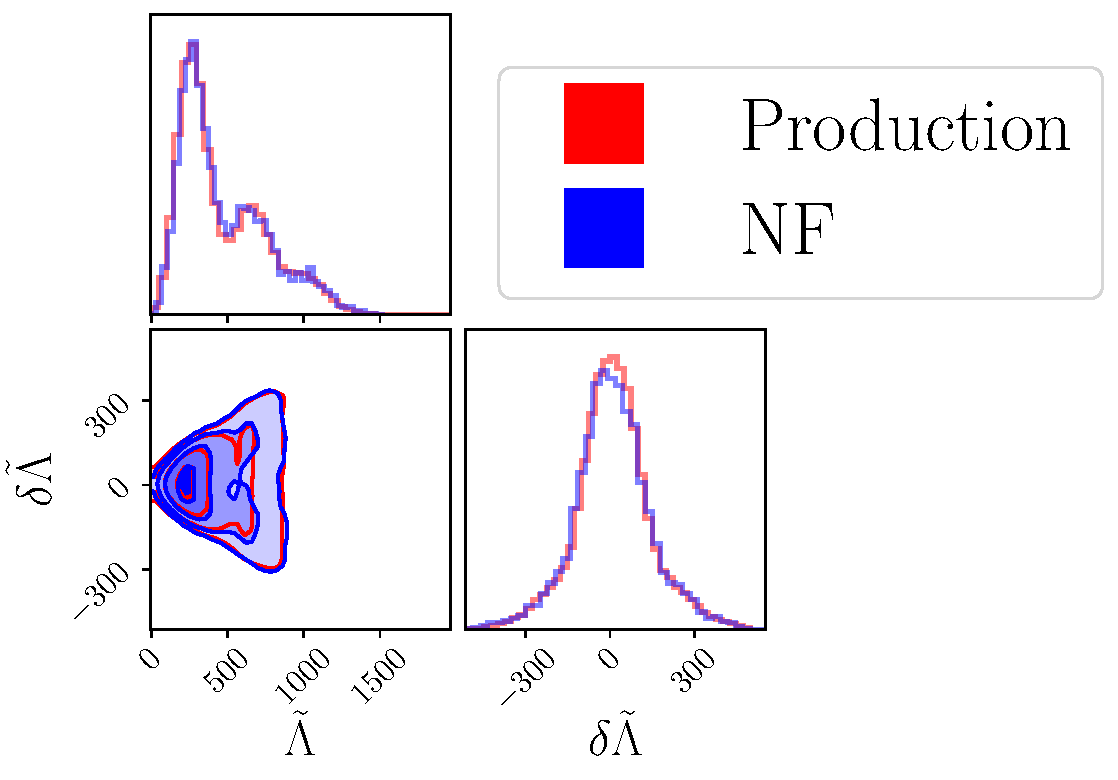
\includegraphics[width = 0.55\textwidth]{Figures/presentation_GW170817_production_vs_NF.pdf}
    \end{figure}
  \end{frame}
  
  
  % \section{Future work \& conclusion}
  
  % \begin{frame}{Future work}
  
  %   \def\x{6mm}
  
  %   \vspace{4mm}
  
  %   \begin{itemize}
  %     \item Finish IMRPhenomD\_NRTidalv2 in \texttt{ripple}
      
  %     \vspace{\x}
      
  %     \item Injection studies and pp-plot
      
  %     \vspace{\x}
  
  %     \item Update NF settings, boost efficiency
      
  %     \vspace{\x}
      
  %     \item Investigate synergy with simulation-based inference (\red{let's talk!})
      
  %     % \vspace{\x}
      
  %     % \item Investigate possibility of pretraining
  %   \end{itemize}
  
  % \end{frame}
  
  % \begin{frame}{Conclusion}
  
  %   \def\x{2mm}
  
  %   \begin{itemize}
  %     \item \texttt{flowMC}: NF-enhanced, gradient-based MCMC
      
  %     \vspace{\x}
      
  %     \item \texttt{ripple}: automatically differentiable GW
      
  %     \vspace{\x}
      
  %     \item $\texttt{jim} = \texttt{jax} + \texttt{flowMC} + \texttt{ripple}$
      
  %     % \vspace{\x}
      
  %     % \item \texttt{jim} is a promising tool for fast and accurate parameter estimation
      
  %     \vspace{\x}
  
  %     \item \texttt{jim} can do PE of BNS in $\sim 1$ min sampling/$\sim 30$ min wall time
      
  %     \vspace{\x}
      
  %     % \item \texttt{jim} can enhance and benefit from simulation-based inference
      
  %   \end{itemize}
  
  %   \vspace{-5mm}
  
  %   \incfig[\textwidth]{jim_flowMC_ripple}
      
  % \end{frame}
  
  % \begin{frame}[plain, noframenumbering]{References}
  
  % \printbibliography
      
  % \end{frame}